%---------------------------------------------------------------------
%
%                          Cap�tulo 4
%
%---------------------------------------------------------------------

\chapter{Aplicando tolerancia a fallos}
\label{trabajotolerancia}

\begin{FraseCelebre}
\begin{Frase}
...
\end{Frase}
\begin{Fuente}
...
\end{Fuente}
\end{FraseCelebre}

\begin{resumen}
En este capitulo se explica c�mo se ha aplicado la tolerancia a fallos en el microprocesador. 
\end{resumen}


%-------------------------------------------------------------------
\section{Introducci�n}
%-------------------------------------------------------------------
\label{trabajotolerancia:introducci�n}

Los fallos m�s comunes en los sistemas electr�nicos son los conocidos como fallos transitorios, estos no da�an el sistema de forma permanente pero provocan un cambio de valor en los elementos de memoria (SEU) o interferencias en las conexiones internas (SET), que si no se estabilizan a tiempo pueden llegar a propagarse hasta una celda de memoria y almacenarse provocando el mismo efecto que un SEU. Con esta informaci�n se ha implementado un m�todo para paliar los efectos de los SEU dentro del microprocesador para reducir los efectos tanto de los SEU como de los SET. 


%------------------------------------------------------------
\section{Redundancia modular}
%------------------------------------------------------------
\label{trabajotolerancia:redundancia}

La t�cnica utilizada para ello ha sido la redundancia modular (NMR) con un valor de $N=3$ . Se ha triplicado cada componente de memoria y se han conectado "`votadores"' a sus salidas. Los "`votadores"' permiten enmascarar una cantidad de fallos igual a $\frac{N}{2}$. En nuestro caso nos permite tolerar un fallo en cada conjunto de m�dulos triplicados. 

Para proporcionar la tolerancia frente a los SEU al sistema, se han sustituido todos los biestables por un conjunto compuesto por tres biestables m�s un votador. Si en principio el sistema conten�a muchos elementos como la figura \ref{fig:Biestable}, ahora estos se han sustituido por el conjunto representado en la figura \ref{fig:BiestablesVotador}.

\begin{figure}[htbp]
  \centering
  \subfloat[Biestable original.\label{fig:Biestable}]{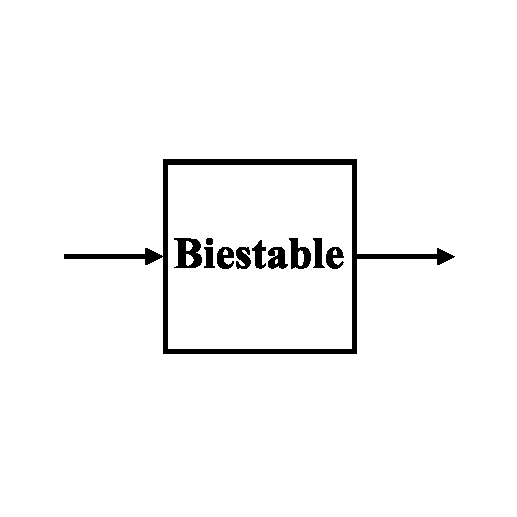
\includegraphics[width=0.45\textwidth]{Imagenes/Tolerancia/Biestable.eps}} \qquad
  \subfloat[Conjunto de biestables con votador.\label{fig:BiestablesVotador}]{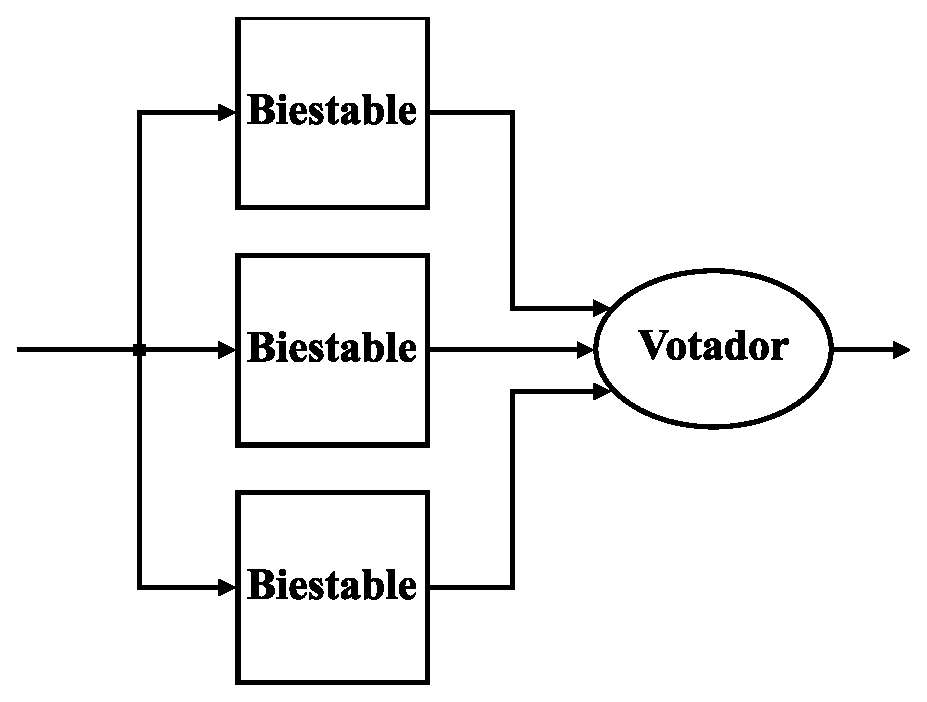
\includegraphics[width=0.45\textwidth]{Imagenes/Tolerancia/BiestablesVotador.eps}}
	\caption{Sustituci�n de biestable.}
\end{figure}


%------------------------------------------------------------
\section{El Votador}
%------------------------------------------------------------
\label{trabajotolerancia:votador}

El votador es un circuito combinacional, y su �nico objetivo es filtrar los valores de entrada, dando un valor de salida igual al de la mayor�a de entradas. Este es el componente principal utilizado para otorgar al sistema de la capacidad de tolerar los fallos transitorios de tipo SEU.

Como se v� en la table \ref{tab:TablaVerdadVotador}, el valor de salida de un votador es igual al valor que m�s se repite en sus entradas. Con este m�todo puede enmascararse un fallo en cualquiera de los m�dulos que alimentan sus entradas.

\begin{table}[ht]
		\centering
			\begin{tabular}{|c|c|c|c|}
			  \hline
				\multicolumn{3}{|c|}{Entradas} & Salida \\ \hline
					A & B & C & Z \\ \hline
					0 & 0 & 0 & 0 \\ \hline
					0 & 0 & 1 & 0 \\ \hline
					0 & 1 & 0 & 0 \\ \hline
					0 & 1 & 1 & 1 \\ \hline
					1 & 0 & 0 & 0 \\ \hline
					1 & 0 & 1 & 1 \\ \hline
					1 & 1 & 0 & 1 \\ \hline
					1 & 1 & 1 & 1 \\ \hline
			\end{tabular}
  \caption{Tabla de verdad del votador}
  \label{tab:TablaVerdadVotador}
\end{table}

La implementaci�n del votador puede realizarse de diferentes formas siempre que cumpla con las restricciones de la tabla \ref{tab:TablaVerdadVotador}. El votador de este proyecto se ha dise�ado siguiendo la f�rmula l�gica \ref{eq:votador}, utilizando con 4 puertas l�gicas, 3 puertas "`AND"' de dos entradas y una puerta "`OR"' de tres entradas. Como se puede observar en la figura \ref{fig:VotadorPuertas},se introduce �nicamente un retardo de 2 puertas l�gicas, haciendo que las puertas l�gicas "`AND"' funcionen en paralelo.

\begin{equation}
  Z = (A*B) + (B*C) + (A*C)
	\label{eq:votador}
\end{equation}

\begin{figure}[ht]
  \centering
	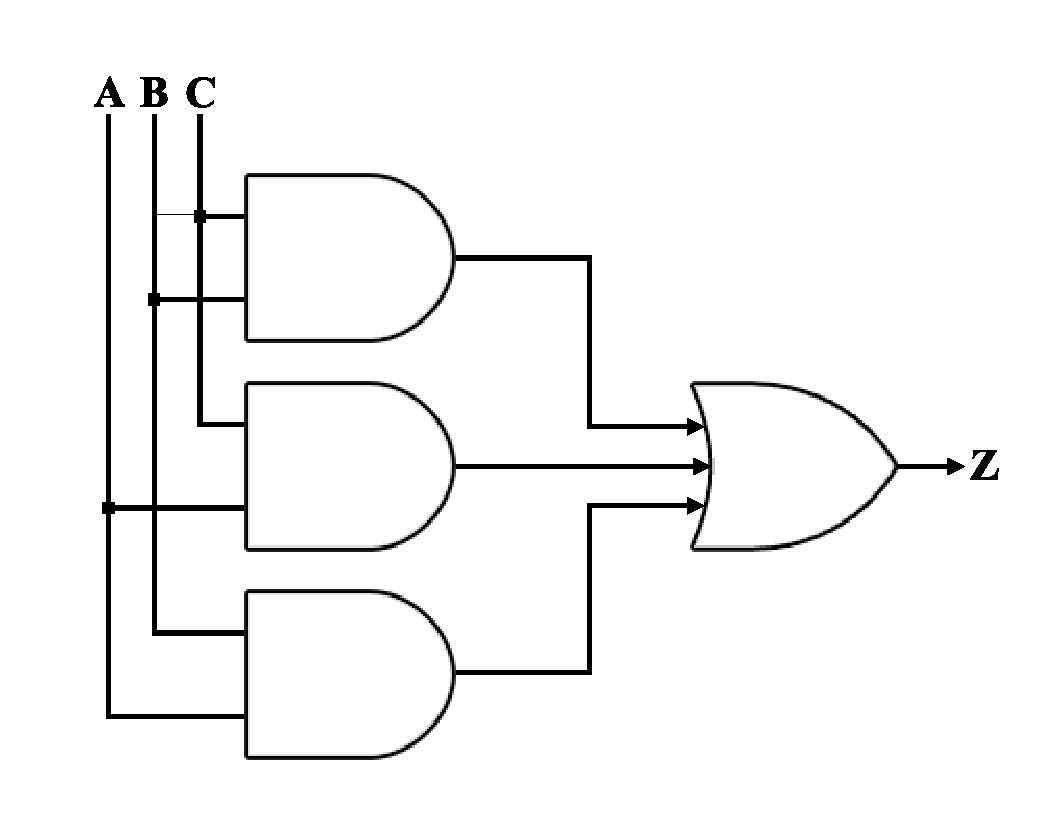
\includegraphics[width=0.50\textwidth]{Imagenes/Tolerancia/VotadorPuertas.eps}
	\caption{Dise�o de votador con puertas l�gicas}
	\label{fig:VotadorPuertas}
\end{figure}

Para exponer c�mo funciona el votador se muestran las figuras \ref{fig:VotadorFalloB} y \ref{fig:VotadorFalloC}. En la figura de la izquierda observamos c�mo la entrada B es diferente al resto, eso quiere decir que el m�dulo origen de esa se�al ha sufrido un fallo. Se observa c�mo se enmascara en las puertas "`AND"' por su funcionalidad ($0 * 1 = 1 * 0 =0$). En el caso de la figura derecha, el fallo ocurre en la entrada C, pero este es enmascarado por la puerta "`OR"'($0 + 0 + 1 = 1$).

\begin{figure}[htbp]
  \centering
  \subfloat[Fallo en entrada B (0 -> 1)\label{fig:VotadorFalloB}]{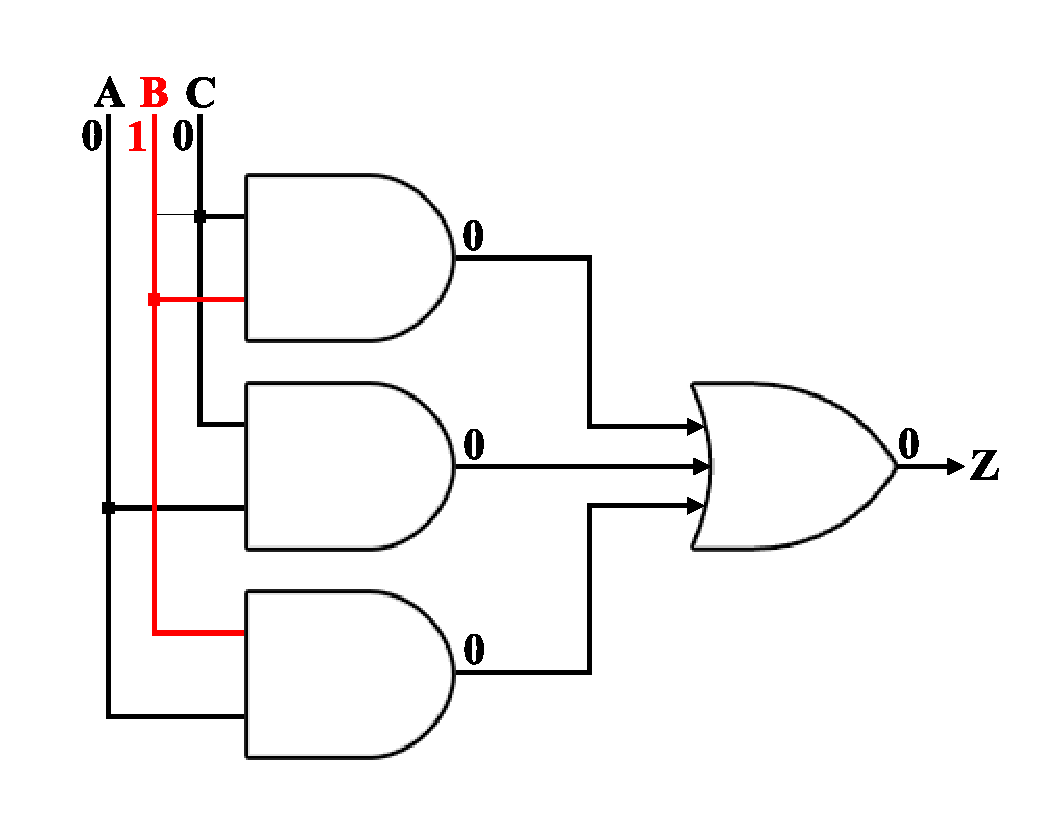
\includegraphics[width=0.45\textwidth]{Imagenes/Tolerancia/FalloB.eps}} \qquad
  \subfloat[Fallo en entrada C (1 -> 0)\label{fig:VotadorFalloC}]{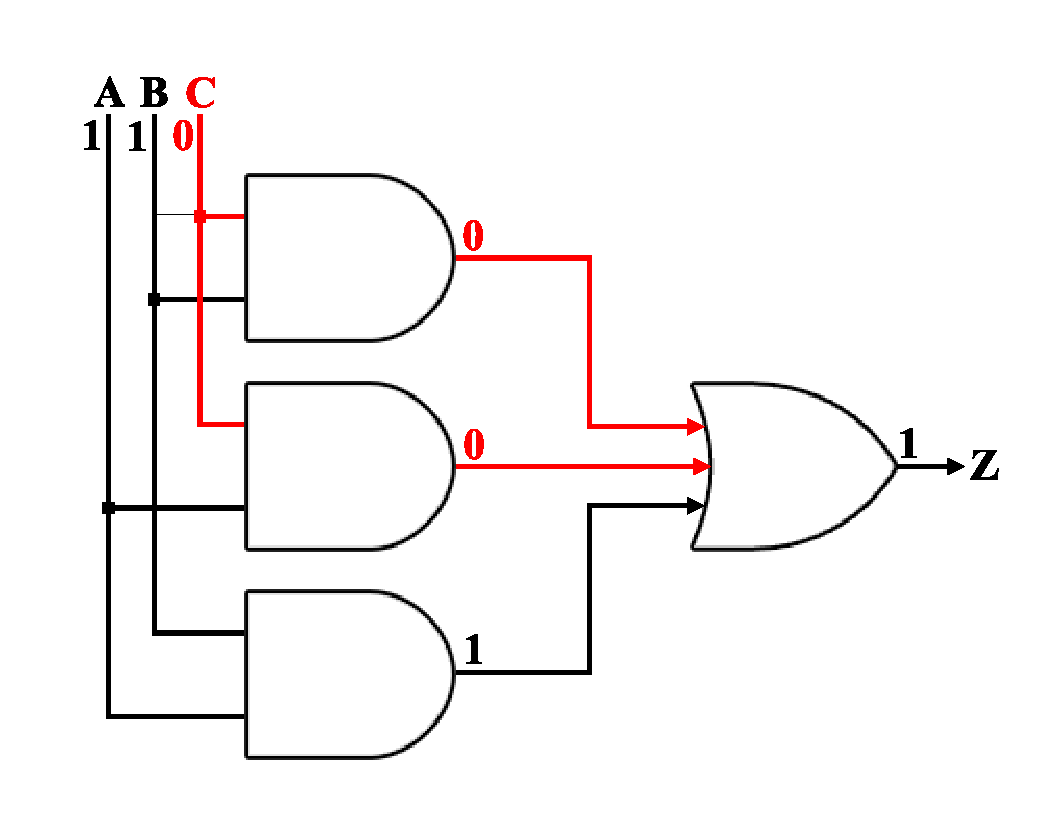
\includegraphics[width=0.45\textwidth]{Imagenes/Tolerancia/FalloC.eps}}
  \caption{Ejemplos de fallos en entradas.}
  \label{fig:VotadorFallos}
\end{figure}

%------------------------------------------------------------
\section{Aplicaci�n}
%------------------------------------------------------------
\label{trabajotolerancia:aplicacion}

La t�cnica de TMR se ha aplicado a cada registro del procesador con la desventaja del aumento en espacio. 
























